%%%%%%%%%%%%%%%%%%%%%%%%%%%%%%%%%%%%%%%%%%%%%%%%%%%%%%%%%%%%%%%%%%%%%%%%%%%
%   Copyright (C) 2011 by Antonio Salvucci                                %
%   s4lb04@gmail.com                                                      %
%                                                                         %
%   This program is free software; you can redistribute it and/or modify  %
%   it under the terms of the GNU General Public License as published by  %
%   the Free Software Foundation; either version 2 of the License.        %
%                                                                         %
%   This program is distributed in the hope that it will be useful,       %
%   but WITHOUT ANY WARRANTY; without even the implied warranty of        %
%   MERCHANTABILITY or FITNESS FOR A PARTICULAR PURPOSE.  See the         %
%   GNU General Public License for more details.                          %
%                                                                         %
%   You should have received a copy of the GNU General Public License     %
%   along with this program; if not, write to the                         %
%   Free Software Foundation, Inc.,                                       %
%   59 Temple Place - Suite 330, Boston, MA  02111-1307, USA.             %
%%%%%%%%%%%%%%%%%%%%%%%%%%%%%%%%%%%%%%%%%%%%%%%%%%%%%%%%%%%%%%%%%%%%%%%%%%%

%%%%%%%%%%%%%%%%%%%%%%%%%%%%%%%
%%%%%%%%%%%%%%%%%%%%%%%%%%%%%%%
\chapter{Index of contents}
\label{ch:Contents}
%%%%%%%%%%%%%%%%%%%%%%%%%%%%%%%
%%%%%%%%%%%%%%%%%%%%%%%%%%%%%%%

%%%%%%%%%%%%%%%%%%%%%%%%%%%%%%%
\section{Main Screen}
\label{sec:ContentsMain}
%%%%%%%%%%%%%%%%%%%%%%%%%%%%%%%

\begin{figure}[h]
  \centering
  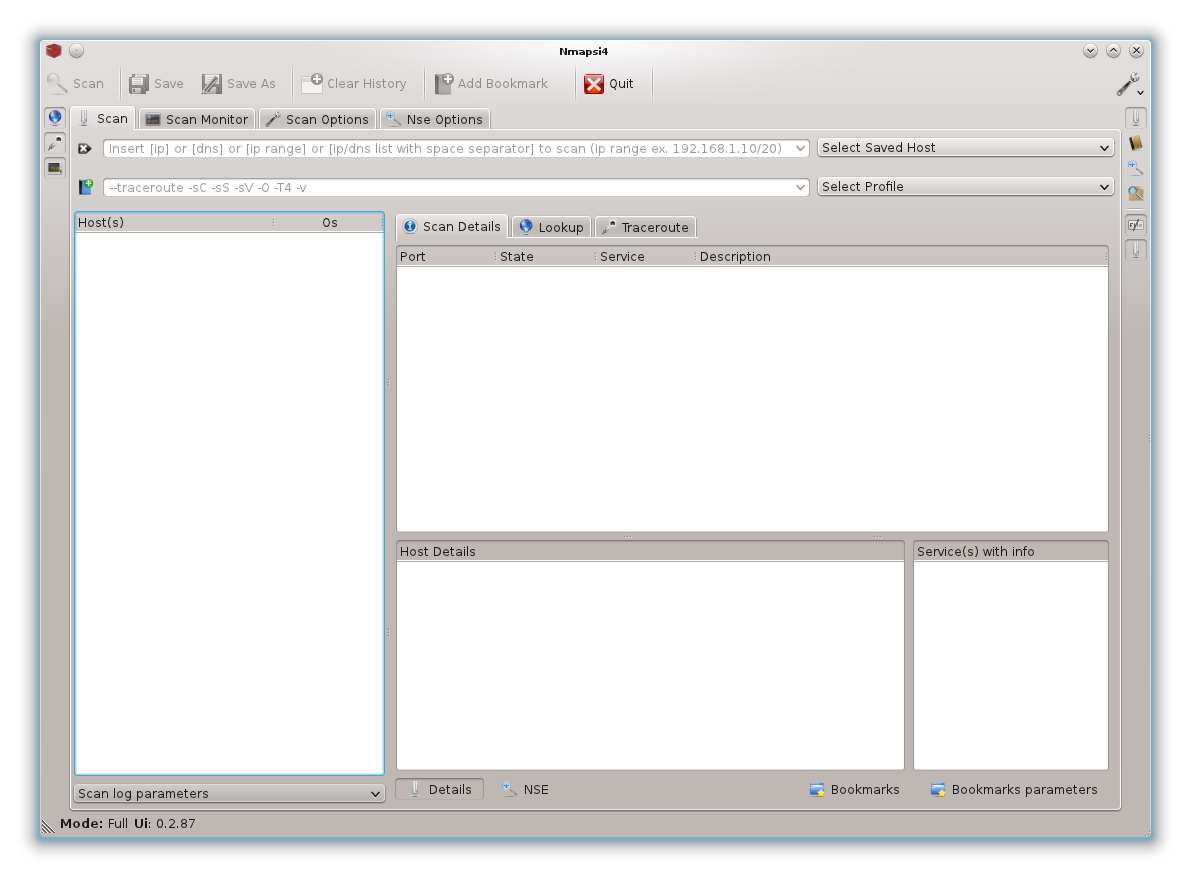
\includegraphics[width=0.65\textwidth]{main}
  \caption{NmapSI4: main screen.}
  \label{fig:ContentsMain}
\end{figure}
This is NmapSI4 main screen, we can notice some elements:
\begin{itemize}
\item Menu bar
\item Toolbar
\item Form for the inclusion of host, ip or dns for scan
\item Form for the inclusion of scan parameters
\item Results screen
\item Statusbar
\end{itemize}
To start a scan you must insert an host, ip or dns, then click on the button
``Scan''. At the end of the scan, in the results screen are visualized scan 
results. On the statusbar you can see with which rights NmapSI4 is working 
together its software version and Nmap software version.

%%%%%%%%%%%%%%%%%%%%%%%%%%
\section{Scanning}
\label{sec:ContentsScan}
%%%%%%%%%%%%%%%%%%%%%%%%%%

This section is about the buttons that you can find under the results screen.

\subsection{Scan details}
\label{sec:ContentsScanScanDetails}

\begin{figure}[h]
  \centering
  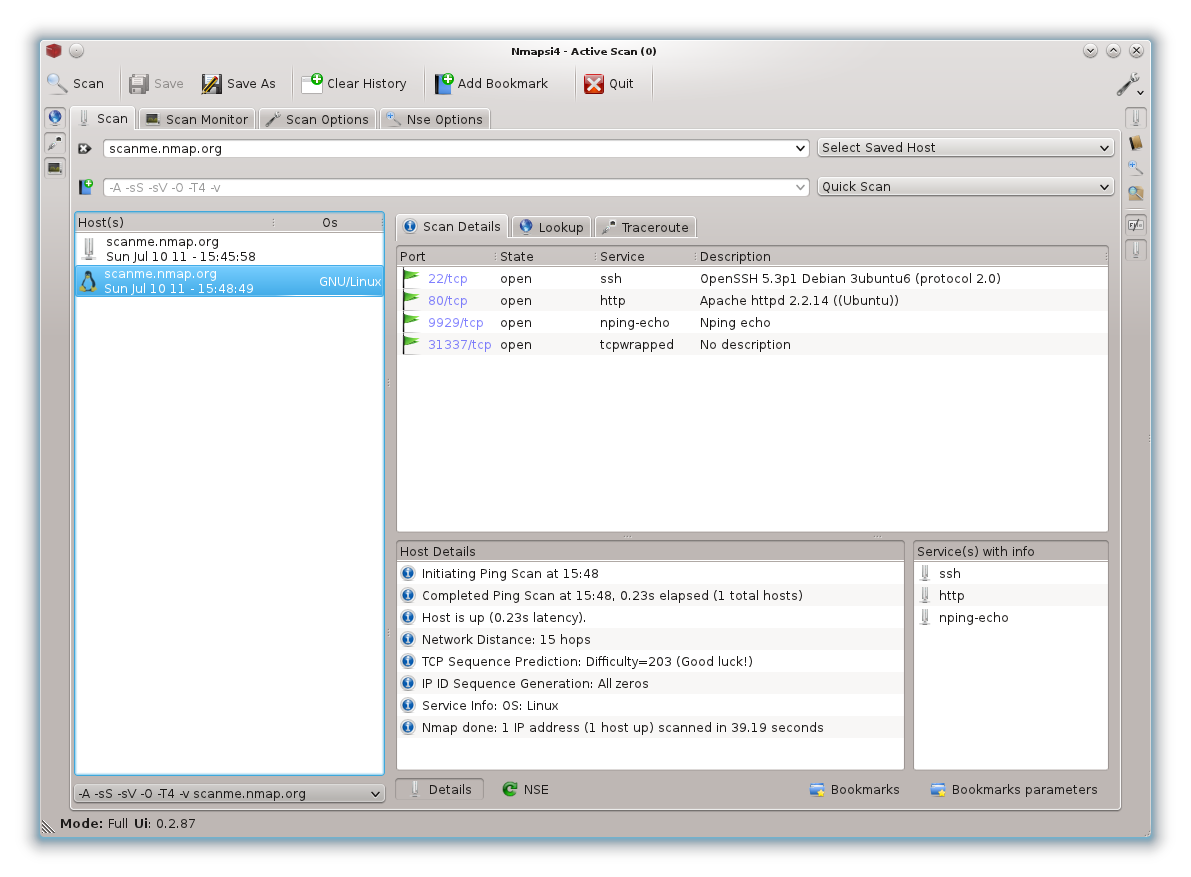
\includegraphics[width=0.65\textwidth]{11scan_details}
  \caption{Scanning: scan details.}
  \label{fig:ContentsScanScanDetails}
\end{figure}
Here there are listed the scan results, and more specifically: service port,
port status, the kind of service and a brief description.

\subsection{Nmap script}
\label{sec:ContentsScanNmapScript}

\begin{figure}[h]
  \centering
  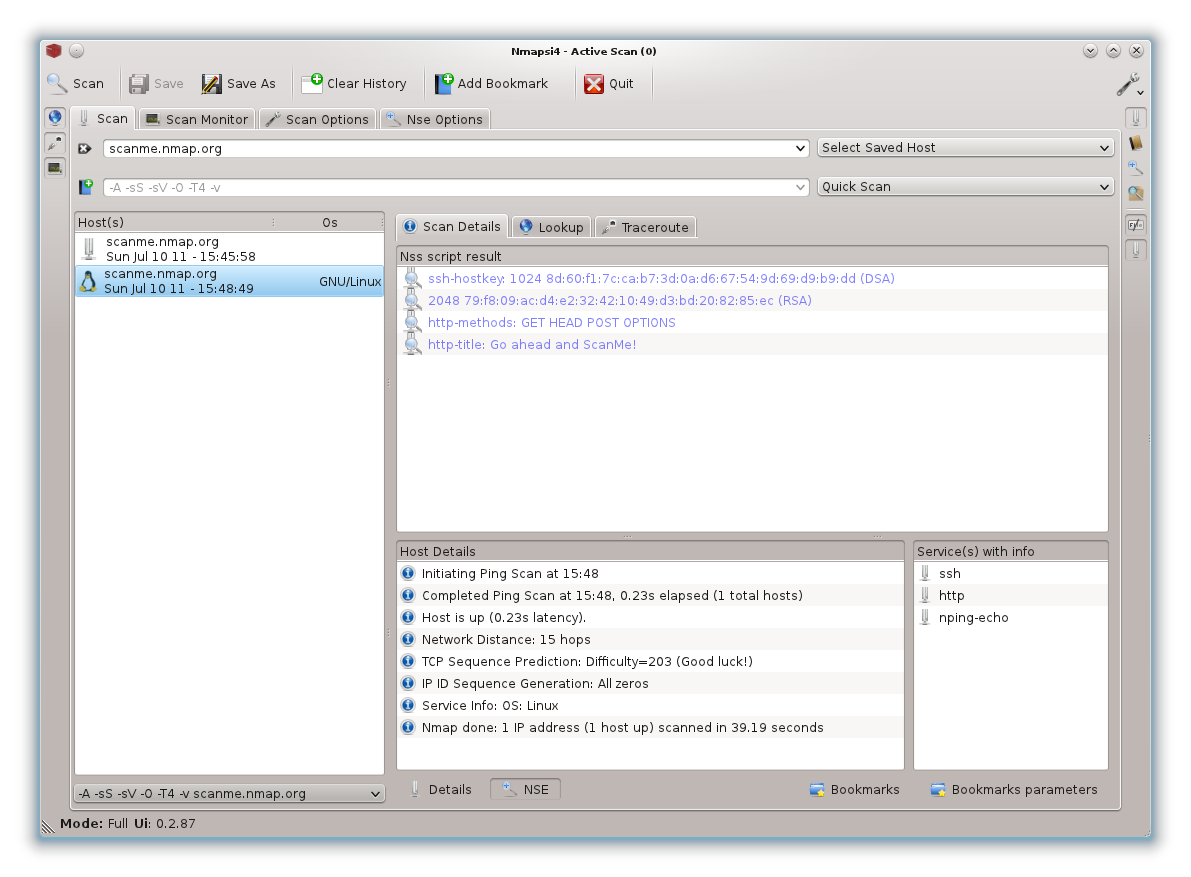
\includegraphics[width=0.65\textwidth]{12nss_result}
  \caption{Scanning: Nmap script.}
  \label{fig:ContentsScanNmapScript}
\end{figure}
Here are showed based on scripts that are part of Nmap Suite. For further 
informations we invite you to look the specific chapter in 
\href{http://nmap.org/book/nse.html}{Nmap}.

\subsection{Host info}
\label{sec:ContentsScanHostInfo}

\begin{figure}[h]
  \centering
  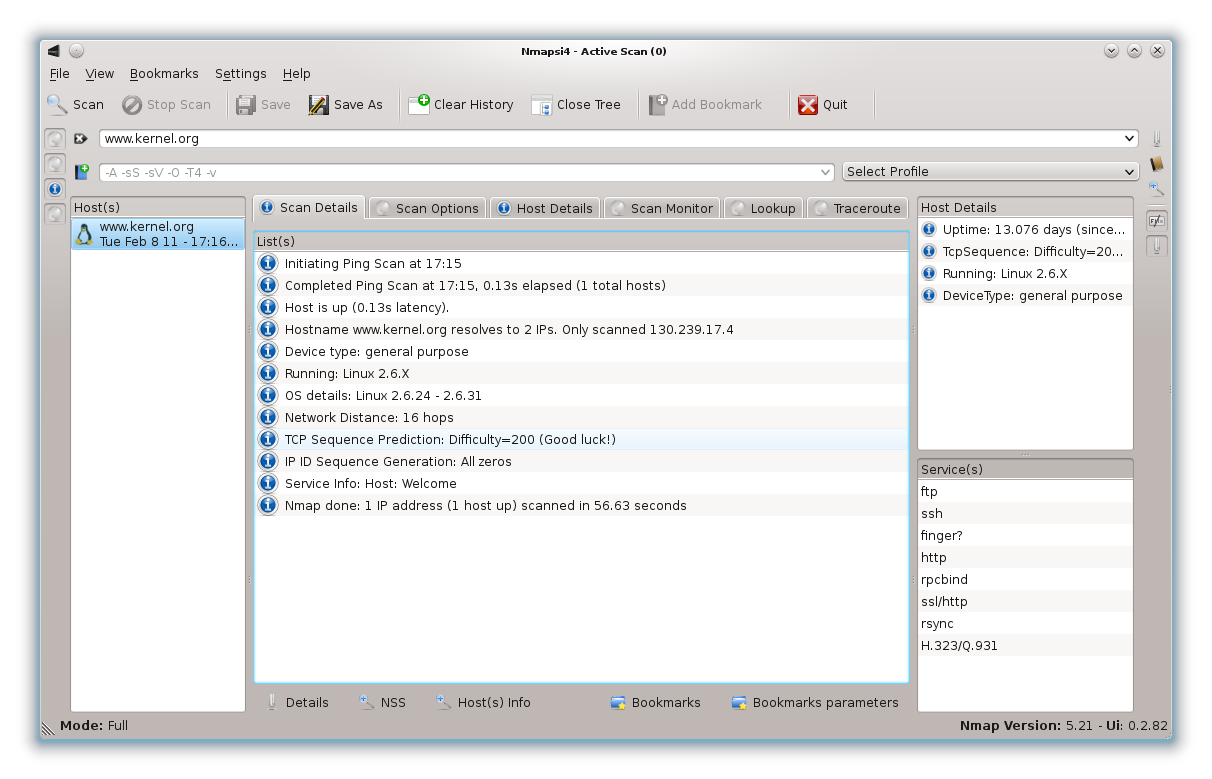
\includegraphics[width=0.7\textwidth]{13host_info}
  \caption{Scanning: host info.}
  \label{fig:ContentsScanHostInfo}
\end{figure}
Here are showed scan details, as the starting time, the duration of scanning 
and other useful informations.

\subsection{Bookmarks}
\label{sec:ContentsScanBookmarks}

\begin{figure}[h]
  \centering
  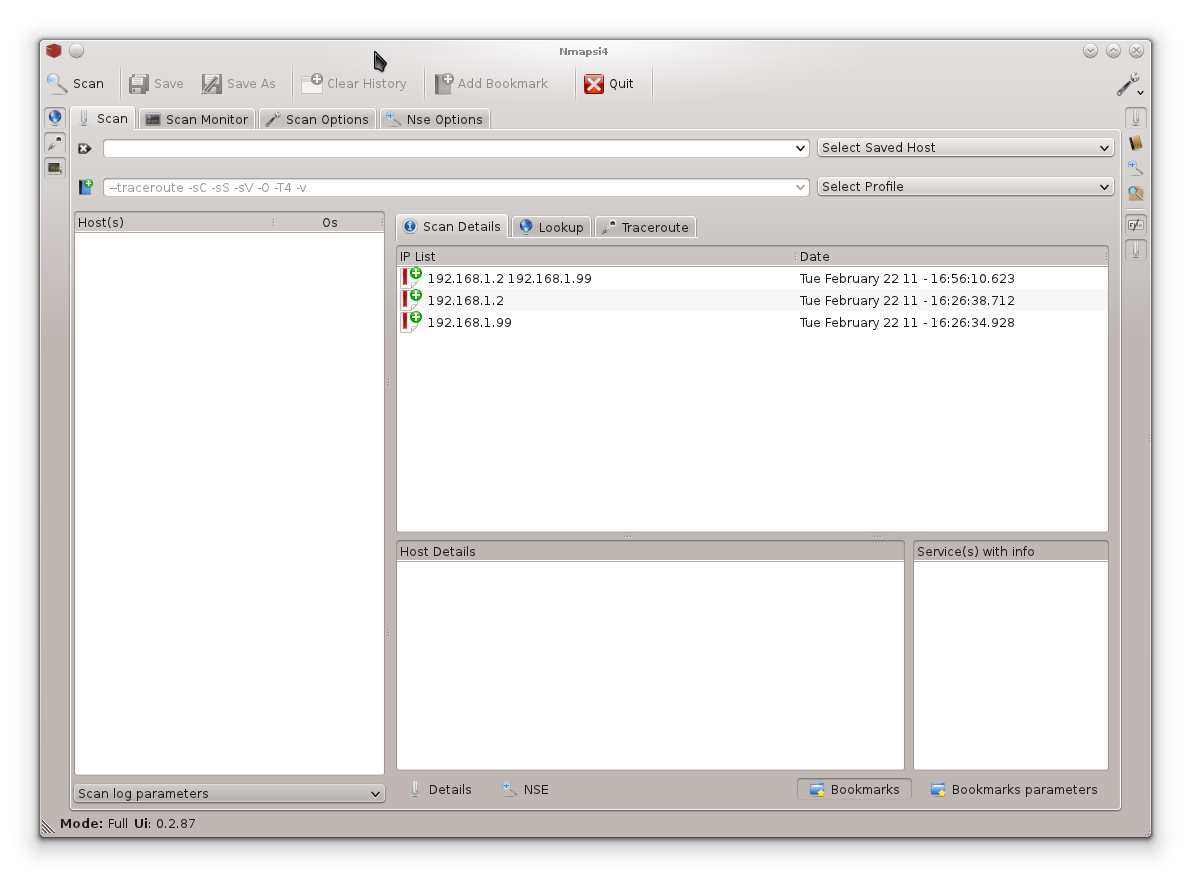
\includegraphics[width=0.7\textwidth]{14bookmarks}
  \caption{Scanning: bookmarks.}
  \label{fig:ContentsScanBookmarks}
\end{figure}
Here we can keep our favourite targets. The screen shows us the ip or the host 
name and the storage date.

\subsection{Bookmarks parameters}
\label{sec:ContentsScanBookmarksParameters}

Here we can see the scan parameters of the stored bookmarks.
\begin{figure}[h]
  \centering
  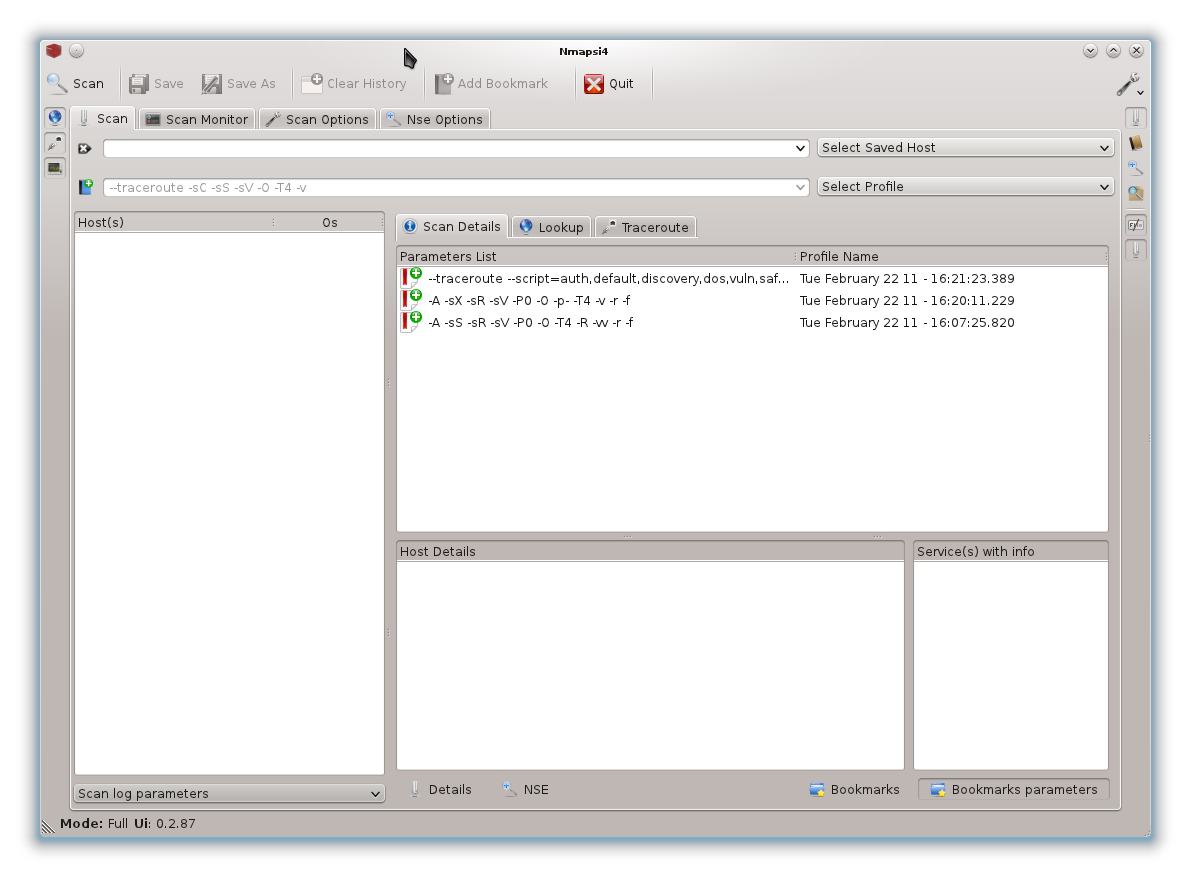
\includegraphics[width=0.7\textwidth]{15bookmarks_parameters}
  \caption{Scanning: bookmarks parameters.}
  \label{fig:ContentsScanBookmarksParameters}
\end{figure}


%%%%%%%%%%%%%%%%%%%%%%%%%%%%%%%%%
\section{Scan options}
\label{sec:ContentsScanOptions}
%%%%%%%%%%%%%%%%%%%%%%%%%%%%%%%%%

In this section you can change scan parameters. To apply changes push the 
``Apply'' button that you find down.

\subsection{Scan}
\label{sec:ContentsScanOptionsScanParameters}

\begin{figure}[h]
  \centering
  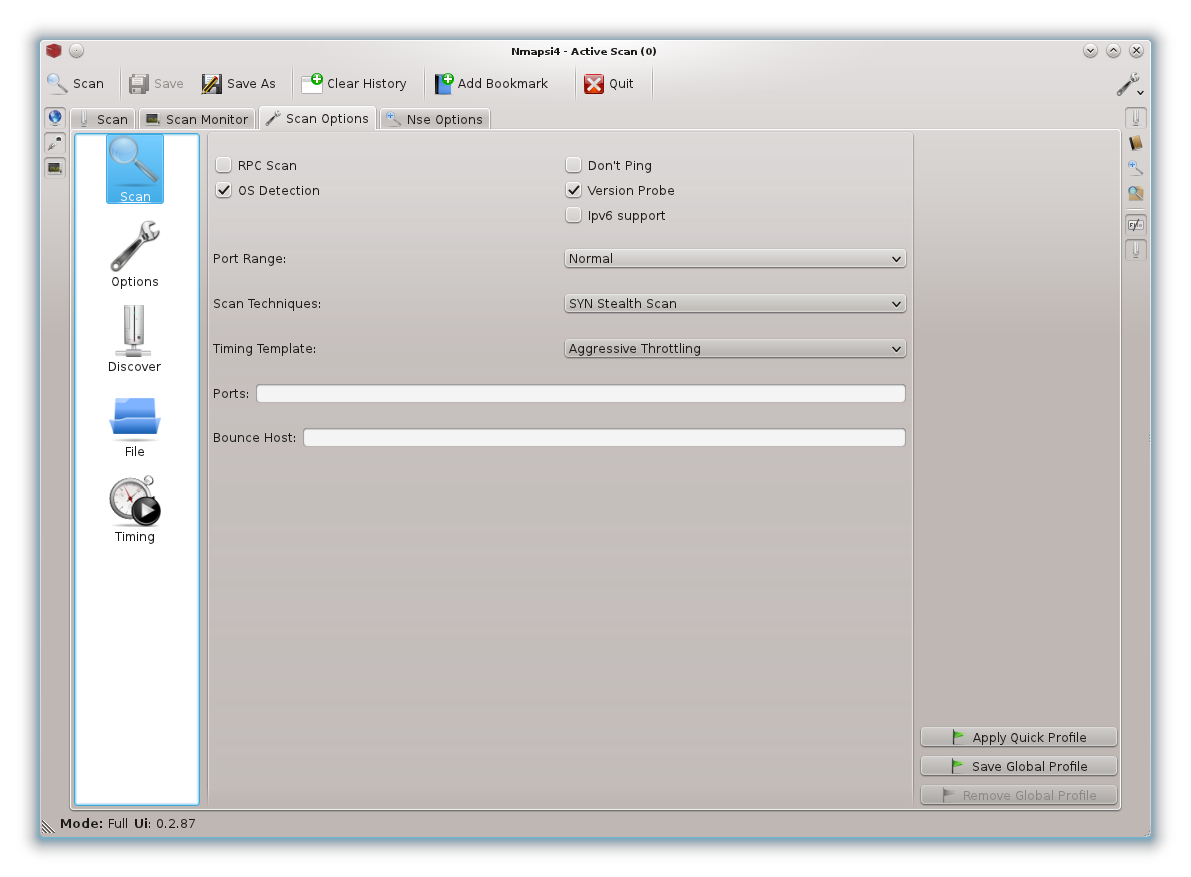
\includegraphics[width=0.7\textwidth]{21scan_options}
  \caption{Scan options: scanning.}
  \label{fig:ContentsScanOptionsScanParameters}
\end{figure}
This section is focused on parameters that stricly concern the scan, just like
profiles, type and number of ports.

\subsection{Options}
\label{sec:ContentsScanOptionsScanParamOptions}

\begin{figure}[h]
  \centering
  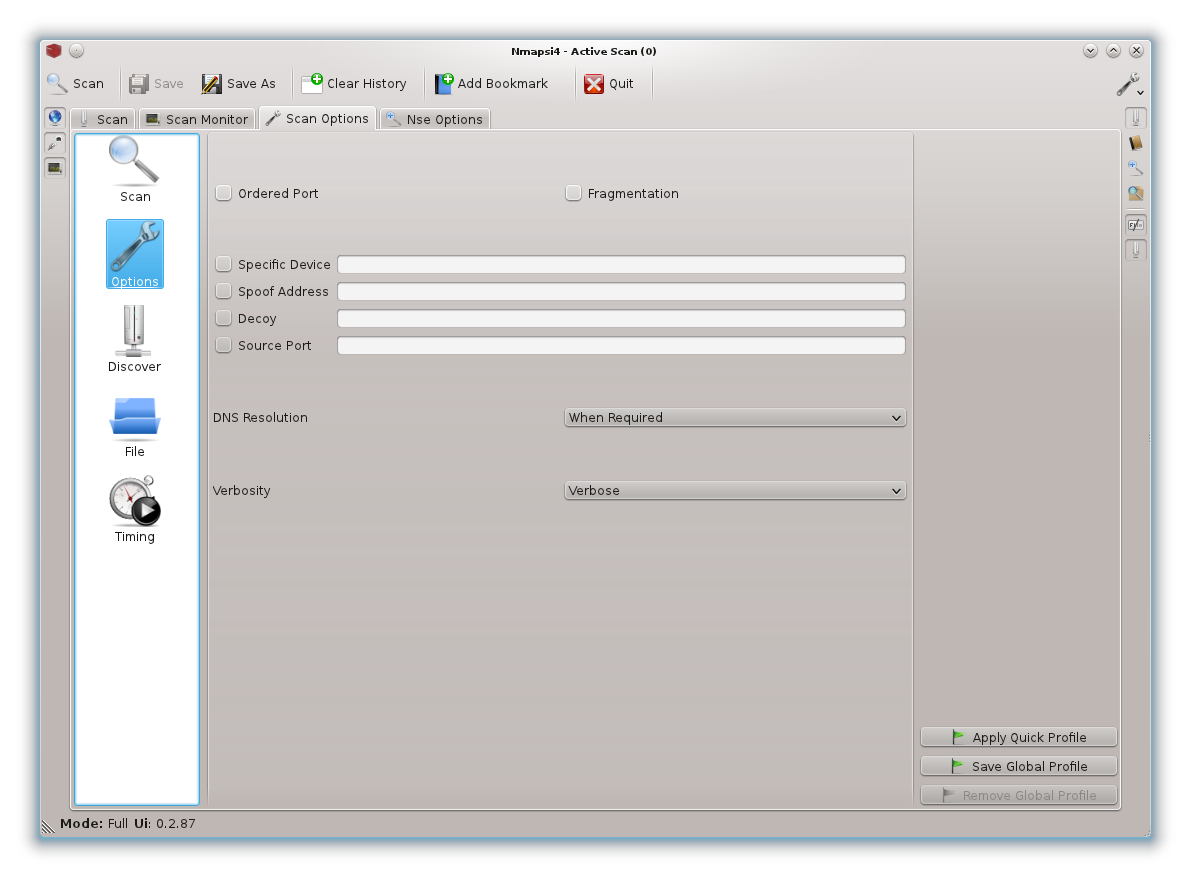
\includegraphics[width=0.7\textwidth]{22scan_options}
  \caption{Scan options: options.}
  \label{fig:ContentsScanOptionsScanParamOptions}
\end{figure}
In this section you can change the detail level and the use of specific
parameters as Ipv6 and fragmentation.

\subsection{Discover}
\label{sec:ContentsScanOptionsScanDiscover}

\begin{figure}[h]
  \centering
  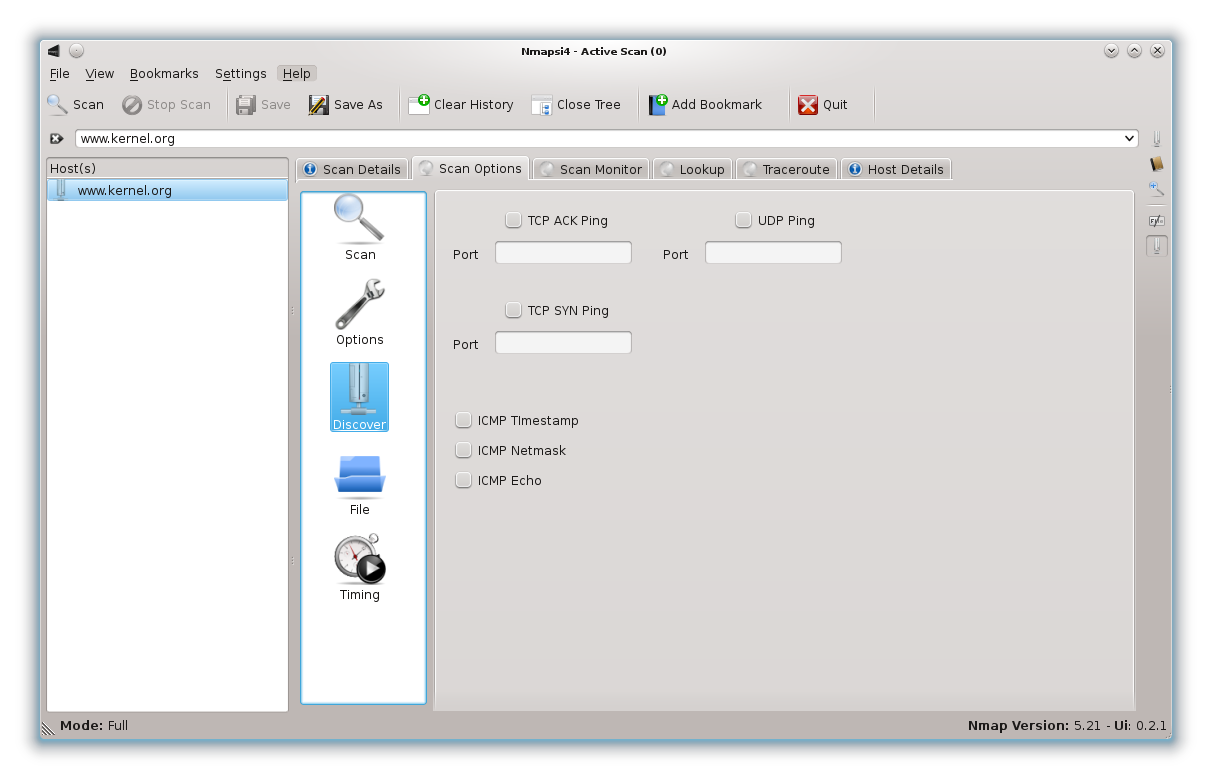
\includegraphics[width=0.7\textwidth]{23discover_scan_options}
  \caption{Scan options: discover.}
  \label{fig:ContentsScanOptionsScanDiscover}
\end{figure}
In this section you can change parameters that concern the type of packets 
that are used in the scan.

\subsection{File}
\label{sec:ContentsScanOptionsScanFile}

\begin{figure}[h]
  \centering
  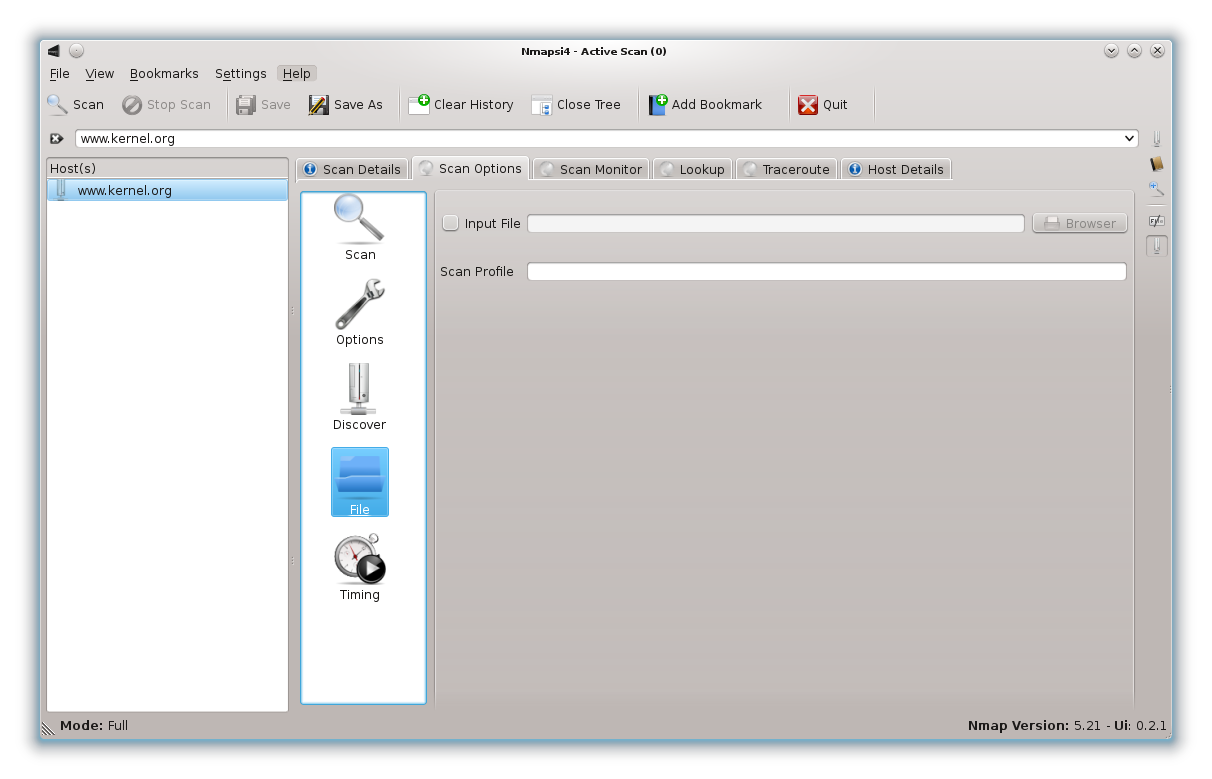
\includegraphics[width=0.7\textwidth]{24file_scan_options1}
  \caption{Scan options: file.}
  \label{fig:ContentsScanOptionsScanFile}
\end{figure}
In this section you can specify an iput file and a specific scan profile.

\subsection{Timing}
\label{sec:ContentsScanOptionsScanTiming}

In this section you can change the parameters that concern the scan time and 
the TTL of send packets.
\begin{figure}[h]
  \centering
  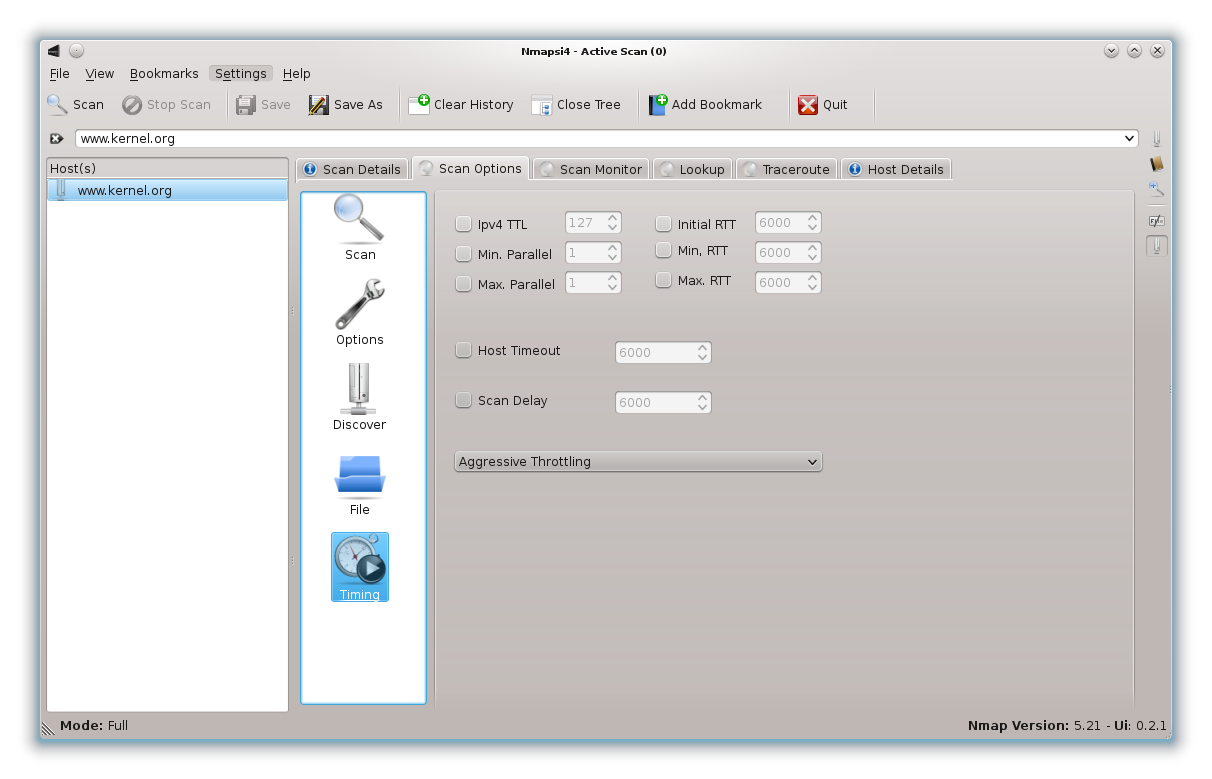
\includegraphics[width=0.7\textwidth]{25timing_scan_options2}
  \caption{Scan options: timing.}
  \label{fig:ConentsScanOptionsScanTiming}
\end{figure}


%%%%%%%%%%%%%%%%%%%%%%%%%%%%%%%%%%%%
\section{Scan monitor}
\label{sec:ContentsScanMonitor}
%%%%%%%%%%%%%%%%%%%%%%%%%%%%%%%%%%%%

\begin{figure}[h]
  \centering
  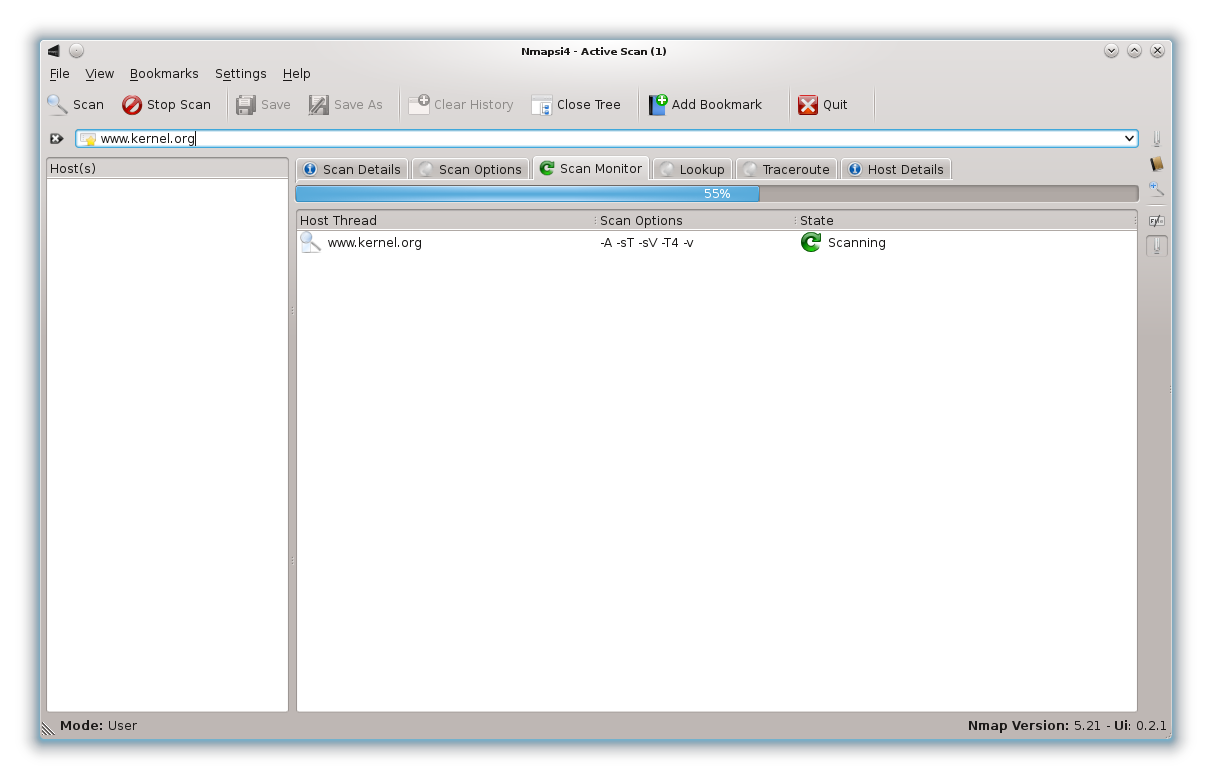
\includegraphics[width=0.7\textwidth]{scan_monitor}
  \caption{Scan monitor.}
  \label{fig:ContentsScanMonitor}
\end{figure}
In this section are listed the several targets of scannings that are active 
and still running.

%%%%%%%%%%%%%%%%%%%%%
\section{Lookup}
\label{sec:ContentsScanMonitorLookup}
%%%%%%%%%%%%%%%%%%%%%

\begin{figure}[h]
  \centering
  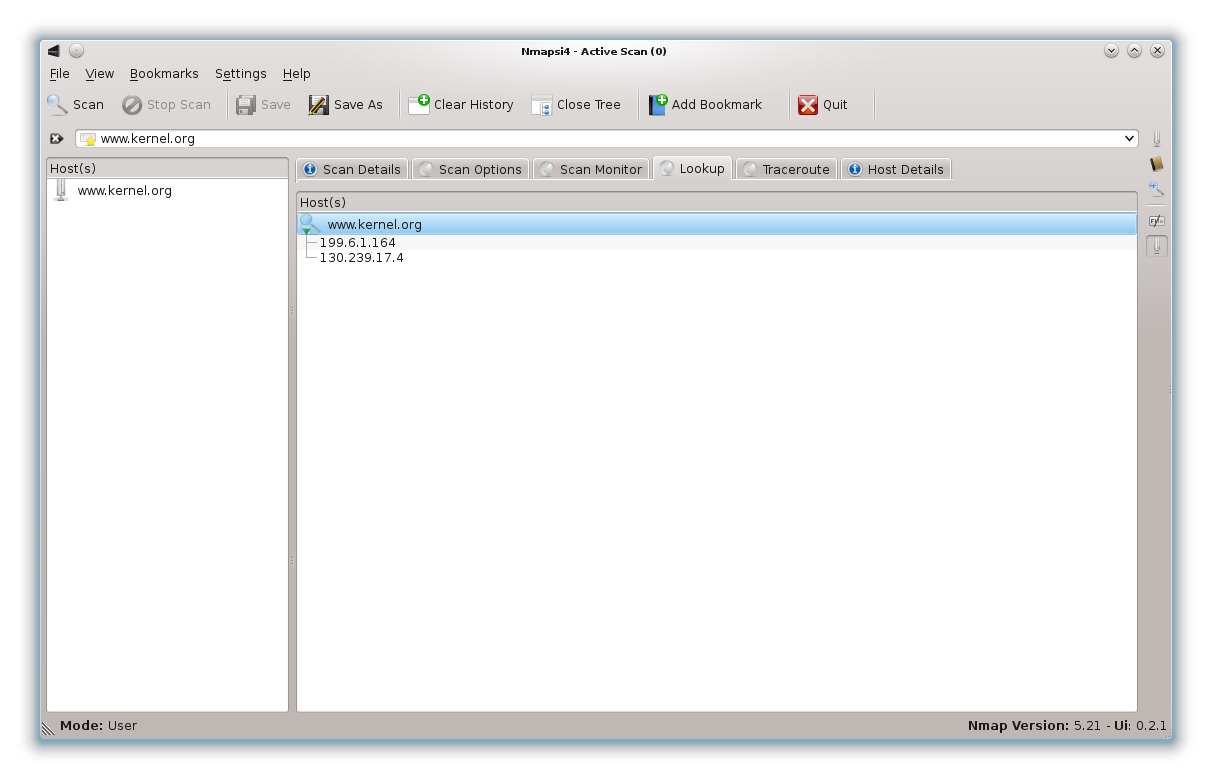
\includegraphics[width=0.7\textwidth]{4scan_lookup}
  \caption{Lookup.}
  \label{fig:ContentsScanMonitorLookup}
\end{figure}
This section shows matches between targets, ip and relates services.

%%%%%%%%%%%%%%%%%%%%%%%%%
\section{Traceroute}
\label{sec:ContentsScanMonitorTraceroute}
%%%%%%%%%%%%%%%%%%%%%%%%%

\begin{figure}[h]
  \centering
  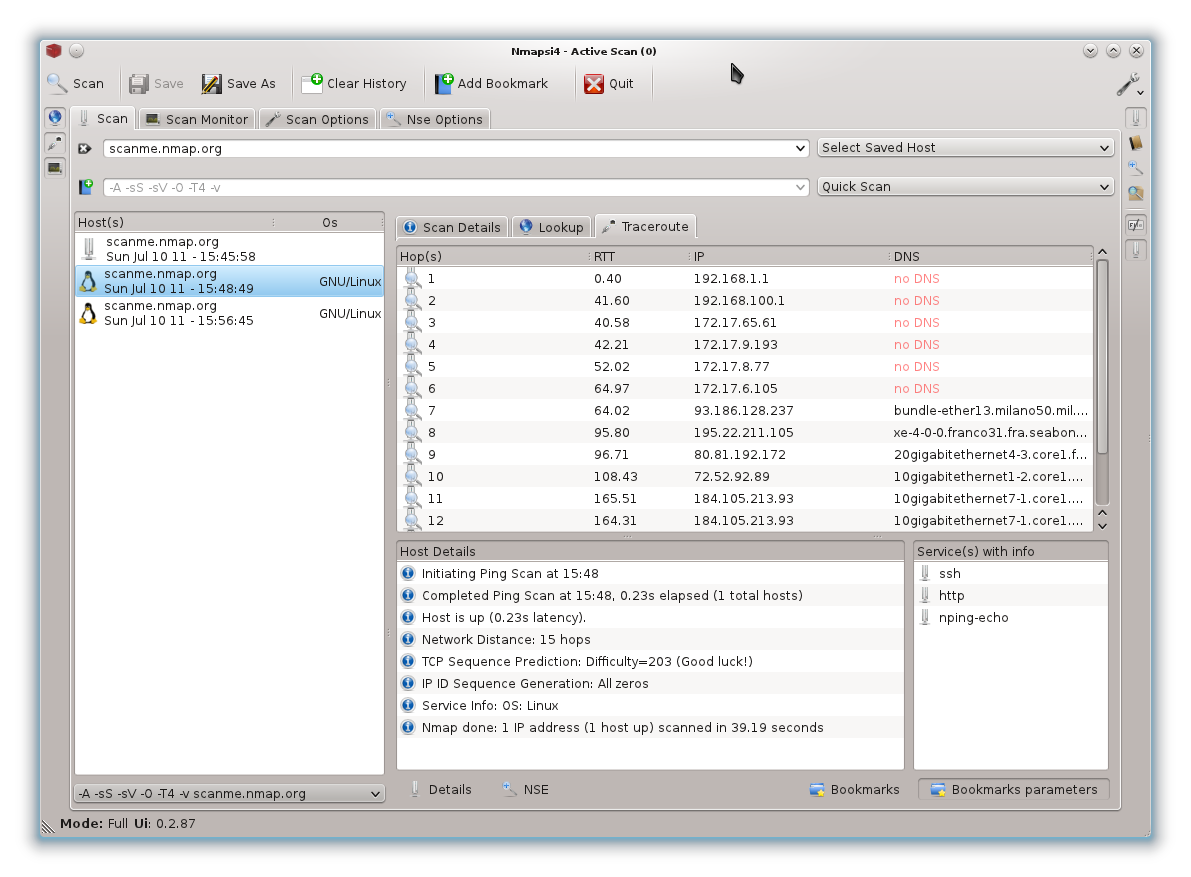
\includegraphics[width=0.7\textwidth]{5traceroute}
  \caption{Traceroute.}
  \label{fig:ContentsScanMonitorTraceroute}
\end{figure}
This section shows the ``route'' followed by scanning packets.

%%%%%%%%%%%%%%%%%%%%%%%%%%%
%%%%%%%%%%%%%%%%%%%%%%%%%%%
\chapter{Preferences}
\label{ch:Preferences}
%%%%%%%%%%%%%%%%%%%%%%%%%%%
%%%%%%%%%%%%%%%%%%%%%%%%%%%

%%%%%%%%%%%%%%%%%%%%%%%%%
\section{Profiles}
\label{sec:Preferencesprofiles}
%%%%%%%%%%%%%%%%%%%%%%%%%

\begin{figure}[h]
  \centering
  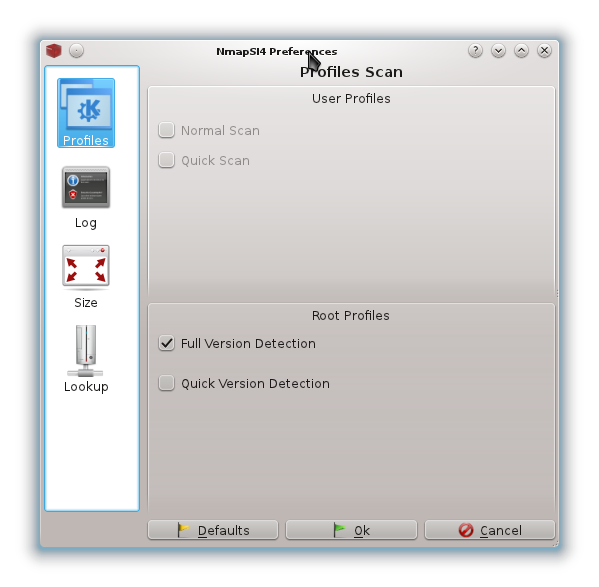
\includegraphics[width=0.6\textwidth]{1preferences_profiles}
  \caption{Preferences: profiles.}
  \label{fig:PreferencesProfili}
\end{figure}
In this section you can change the predefined scan profile.

%%%%%%%%%%%%%%%%%%%
\section{Log}
\label{sec:PreferencesLog}
%%%%%%%%%%%%%%%%%%%

\begin{figure}[h]
  \centering
  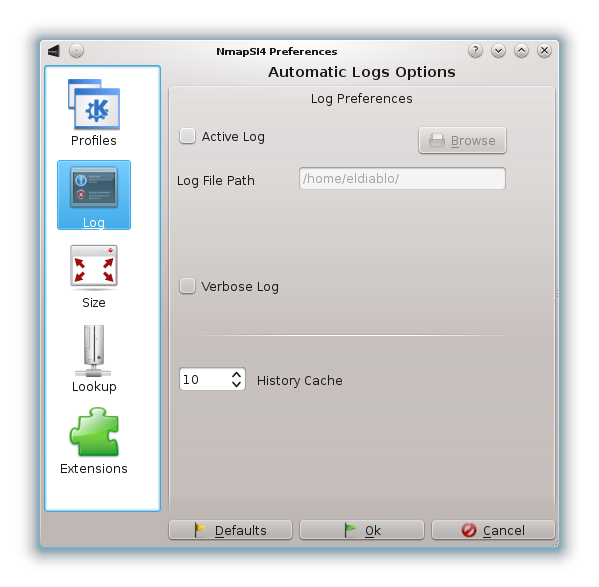
\includegraphics[width=0.6\textwidth]{2preferences_log}
  \caption{Preferences: log.}
  \label{fig:PreferencesLog}
\end{figure}
In this section you can change the settings of scannings log.

%%%%%%%%%%%%%%%%%%%%%%%%%
\section{Sizes}
\label{sec:PreferencesDimensions}
%%%%%%%%%%%%%%%%%%%%%%%%%

\begin{figure}[h]
  \centering
  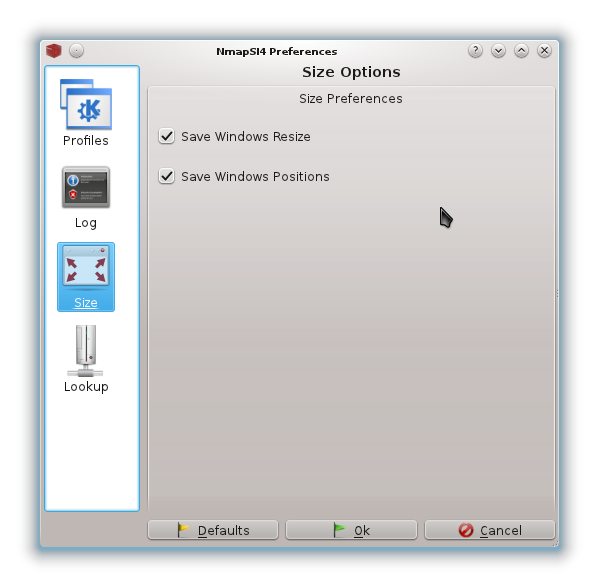
\includegraphics[width=0.6\textwidth]{3preferences_size}
  \caption{Preferences: sizes.}
  \label{fig:PreferencesDimensions}
\end{figure}
In this section you can change settings of NmapSI4 main window.

%%%%%%%%%%%%%%%%%%%%%%%%%%%%%%%
\section{Lookup}
\label{sec:PreferencesLookup}
%%%%%%%%%%%%%%%%%%%%%%%%%%%%%%%

\begin{figure}[h]
  \centering
  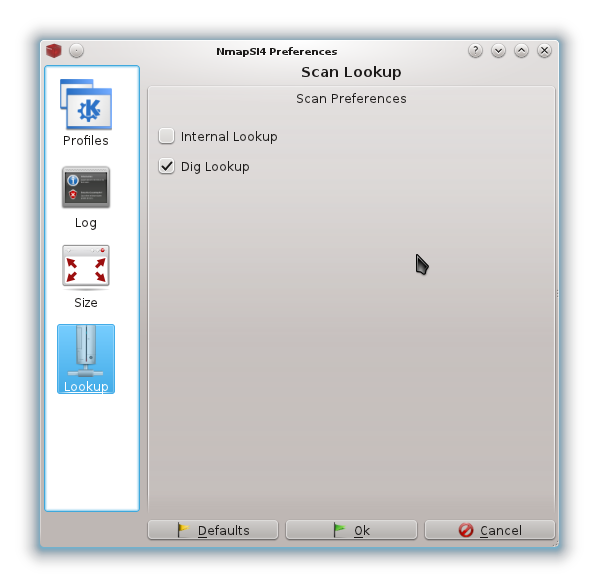
\includegraphics[width=0.6\textwidth]{4preferences_lookup}
  \caption{Preferences: lookup.}
  \label{fig:PreferencesLookup}
\end{figure}
In this section you can change lookup settings.

%%%%%%%%%%%%%%%%%%%%%%%%%%%%%%%%%%
\section{Extensions}
\label{sec:PreferencesExtensions}
%%%%%%%%%%%%%%%%%%%%%%%%%%%%%%%%%%

\begin{figure}[h]
  \centering
  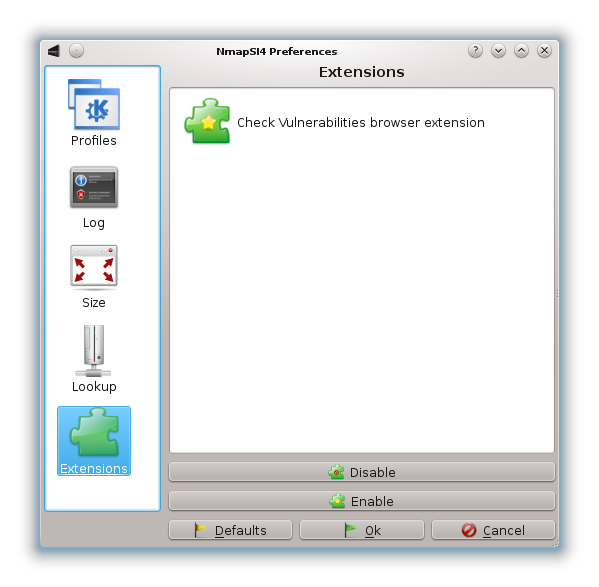
\includegraphics[width=0.6\textwidth]{5preferences_extensions}
  \caption{Preferences: extensions.}
  \label{fig:PreferencesExtensions}
\end{figure}
In this section you can enable or disable NmapSI4 extensions.

%%%%%%%%%%%%%%%%%%%%%%%%%%%%%%%%%%%%%%%%%%%%%%%%%
%%%%%%%%%%%%%%%%%%%%%%%%%%%%%%%%%%%%%%%%%%%%%%%%%
\chapter{Vulnerabilities search engine}
\label{ch:Vulnerability}
%%%%%%%%%%%%%%%%%%%%%%%%%%%%%%%%%%%%%%%%%%%%%%%%%
%%%%%%%%%%%%%%%%%%%%%%%%%%%%%%%%%%%%%%%%%%%%%%%%%

%%%%%%%%%%%%%%%%%%%%%%%%%%%%%%%%%%
\section{Main screen}
\label{sec:VulnerabilityMain}
%%%%%%%%%%%%%%%%%%%%%%%%%%%%%%%%%%

\begin{figure}[h]
  \centering
  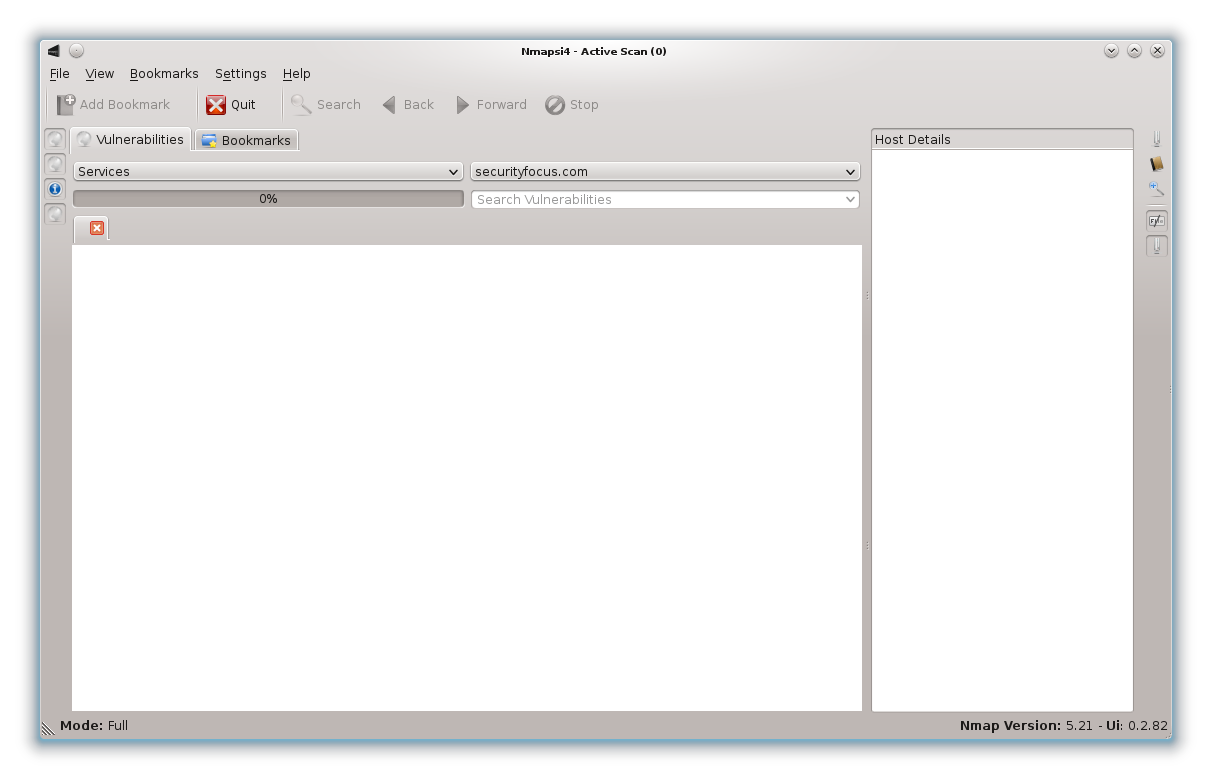
\includegraphics[width=0.7\textwidth]{vulnerabilities}
  \caption{Vulnerabilities search engine: main screen.}
  \label{fig:VulnerabilityMain}
\end{figure}
This section provides a search engine to look for possible vulnerabilities of 
services traced during the scan, within the best reference sites about 
vulnerabilities. You can plan the research depending on the specific service 
recognized during the scanning, or you can choose another search key.


%%%%%%%%%%%%%%%%%%%%%%%%%%%%%%%%%%%%%%
\section{Bookmarks}
\label{sec:VulnerabilityBookmarks}
%%%%%%%%%%%%%%%%%%%%%%%%%%%%%%%%%%%%%%

\begin{figure}[h]
  \centering
  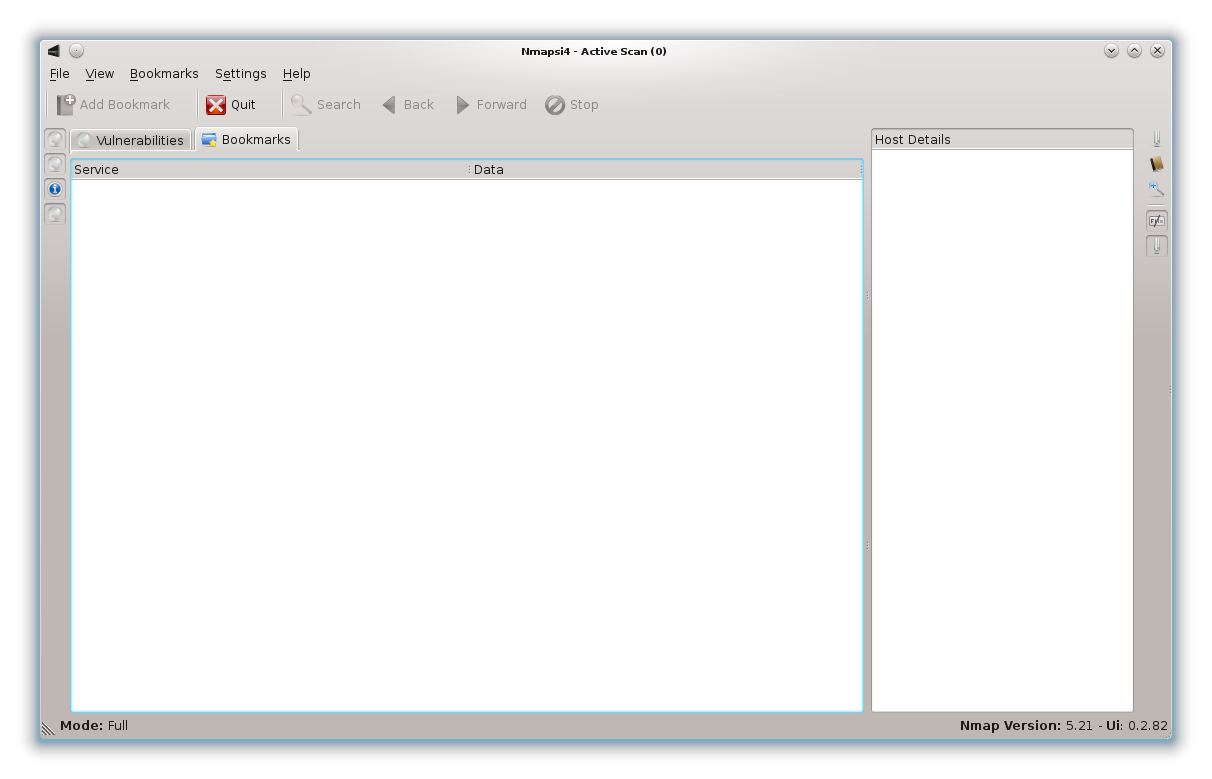
\includegraphics[width=0.7\textwidth]{vuln_bookmarks}
  \caption{Vulnerabilities search engine: bookmarks.}
  \label{fig:VulnerabilityBookmarks}
\end{figure}
Here you can memorize your favourite results.


%%%%%%%%%%%%%%%%%%%%%%%%%%%%%%
%%%%%%%%%%%%%%%%%%%%%%%%%%%%%%
\chapter{Log reader}
\label{ch:LogReader}
%%%%%%%%%%%%%%%%%%%%%%%%%%%%%%
%%%%%%%%%%%%%%%%%%%%%%%%%%%%%%

%%%%%%%%%%%%%%%%%%%%%%%%%%%%%%%%%%%%
\section{Main screen}
\label{sec:LogReaderMainScreen}
%%%%%%%%%%%%%%%%%%%%%%%%%%%%%%%%%%%%

\begin{figure}[h]
  \centering
  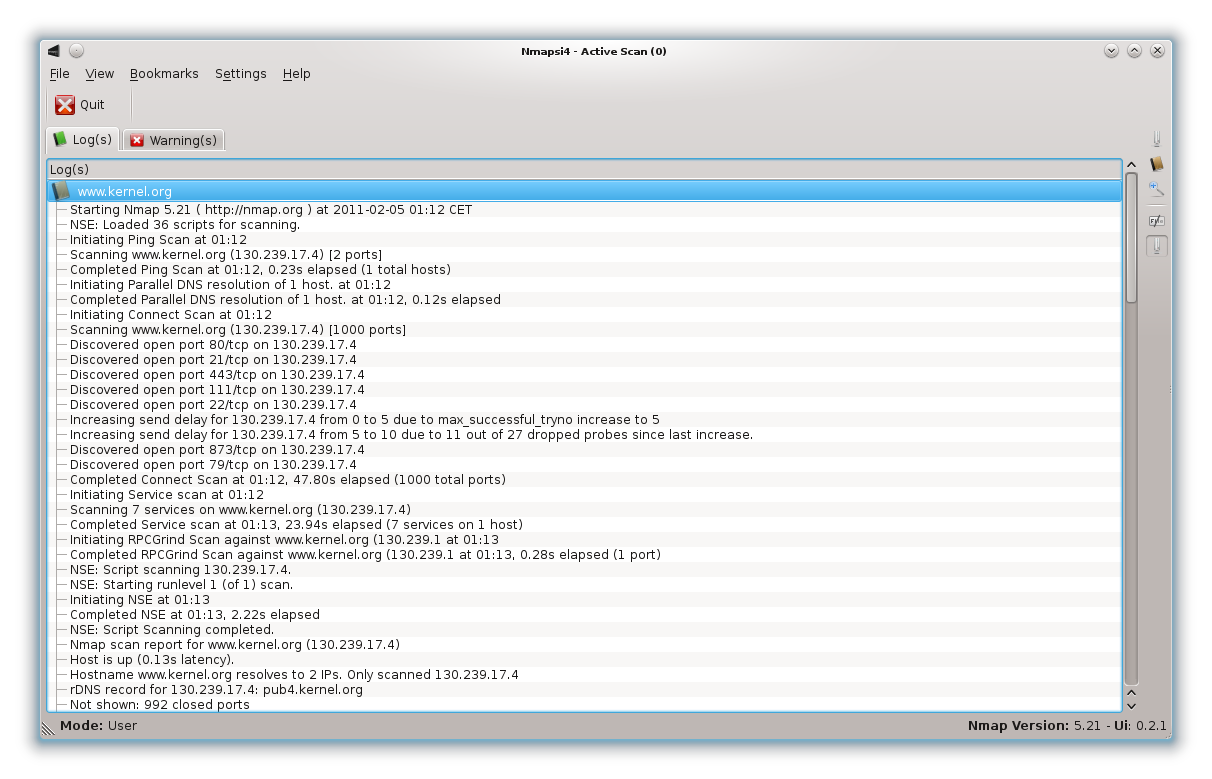
\includegraphics[width=0.7\textwidth]{log_reader}
  \caption{Log reader: main screen.}
  \label{fig:LodReader}
\end{figure}
This section allowes you to read the complete output of Nmap scan.


%%%%%%%%%%%%%%%%%%%%%%%%%%%%%%%%%%%
%%%%%%%%%%%%%%%%%%%%%%%%%%%%%%%%%%%
\chapter{Some examples}
\label{ch:Examples}
%%%%%%%%%%%%%%%%%%%%%%%%%%%%%%%%%%%
%%%%%%%%%%%%%%%%%%%%%%%%%%%%%%%%%%%

%%%%%%%%%%%%%%%%%%%%%%%%%%%%%%%%%%%%%%
\section{Multiple scannings}
\label{sec:ExamplesMultipleScan}
%%%%%%%%%%%%%%%%%%%%%%%%%%%%%%%%%%%%%%

You can use scannings in different ways:
\begin{itemize}
\item single scanning: \emph{ip (e.g. 192.168.1.1) or dns (es. www.kernel.org)}
\item multiple scanning: \emph{range di ip (e.g. 192.168.1.10/20) to scan from
  192.168.1.10 to 192.168.1.20}
\item ip and dns mixed scanning: \emph{e.g. 192.168.1.1 www.kernel.org}
\item scan on an ip or dns list: \emph{e.g. 192.168.1.10 192.168.1.15,
  or www.kernel.org www.google.com}
\end{itemize}
\textbf{It's preferable not to insert and high hosts number to scan}.

%%%%%%%%%%%%%%%%%%%%%%%%%%%%%%%%%%%%%%
\section{Using bookmarks}
\label{sec:ExamplesUseBookmarks}
%%%%%%%%%%%%%%%%%%%%%%%%%%%%%%%%%%%%%%

For using bookmarks, just push the button up to add it to the list.\\
In the same way to save the scanning profile there's the button placed near 
the parameters input form.\\
To reuse later an host or a saved profile, just select it in the related 
screen and choose ``Scanning'' for hosts or ``Use parameters'' for profiles.\\
To remove an entry from the list, repeat the reuse procedure, choosing the 
clearing entry.
